\chapter{Vorauswahl}
Um die möglichen Optionen einzugrenzen wird im folgenden eine Auflistung der Topologien erstellt und anhand einfacher Kriterien die Auswahl eingegrenzt. Einen guten Überblick über Schaltungen für Dreiphasige Gleichrichter mit Leistungsfaktorkorrektur gibt die Präsentation von Dominik Bortis et al. \cite{Advanced3PhPFC}. Diese bezieht sich auf Systeme mit aktiver Leistungsfaktorkorrektur. Aufgrund gewünschter Systemdienstleistungen, wie Blindleistungsbereitstellung sind Systeme mit Hybrider Kompensation nicht ausreichend.


\section{Mögliche Topologien}
Die Grundlegende Topologie welche zur Vollständigkeit aufgelistet wird, ist der dreiphasige Diodengleichrichter, welcher bereits in Abschnitt \ref{sec:Rec} dargestellt wurde. Die weiteren Topologien werden im folgenden aufgelistet.
	\subsection{6-Switch Boost PFC Rectifier}
			Bei der ersten Topologie wurde prinzipiell beim Diodengleichrichter, die Dioden durch Schalter ersetzt, siehe Abbildung \ref{fig:sixswitchboost} Dies ermöglicht im Zusammenspiel mit den Eingangsimpedanzen ein Hochstellendes verhalten und Modulation der Eingangsströme über verschiedene \gls{PWM} Verfahren zum gewünschten Sinusförmigen Eingangsstrom.
			\begin{figure}
				\centering
				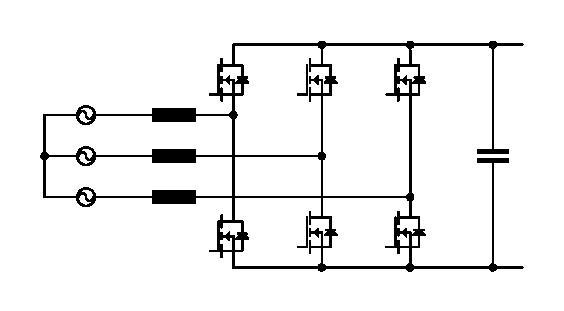
\includegraphics[width=0.7\linewidth]{content/Grafiken/SixSwitchBoost}
				\caption{Six Switch Boost PFC Rectifier}
				\label{fig:sixswitchboost}
			\end{figure}
			
	\subsection{Vienna Rectifier}
		Hierbei handelt es sich ebenfalls um eine Hochstellende Topologie. Diese besteht aus einem Diodengleichrichter mit Eingangsinduktivitäten und wird ergänzt durch einen \gls{IVS} an welchen Kapazitäten zur Ausgangsspannung geschaltet werden können. Siehe Abbildung \ref{fig:vienna}. Durch diese 3-Level Struktur, kann eine bessere Form des Eingangsstroms erreicht werden, als bei der 2-Level 6-Switch Boost PFC Topologie. Außerdem kann aus selbem Grund die Induktivität kleiner ausfallen.
		\begin{figure}
			\centering
			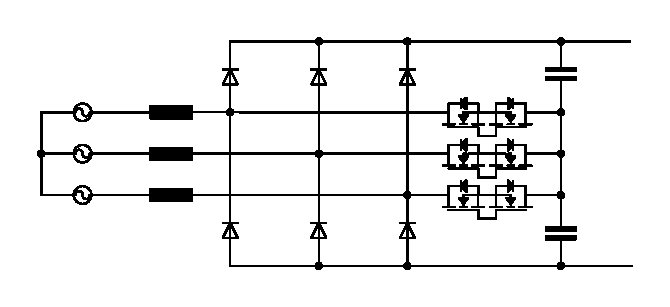
\includegraphics[width=0.7\linewidth]{content/Grafiken/Vienna}
			\caption{Vienna Rectifier}
			\label{fig:vienna}
		\end{figure}
		
	\subsection{6-Switch Buck PFC Rectifier}
		Durch verschieben der Drossel auf die Ausgangsseite entsteht aus dem 6-Switch Boost eine Tiefstellende Topologie. Jedoch wird sperrendes Verhalten in beide Richtungen benötigt, um die Ausgangsspannung und den Eingangsstrom in die gewünschte Form zu bringen. Daher werden die Schalter durch Dioden ergänzt, wie in Abbildung \ref{fig:sixswitchbuck} dargestellt. 
		
		\begin{figure}
			\centering
			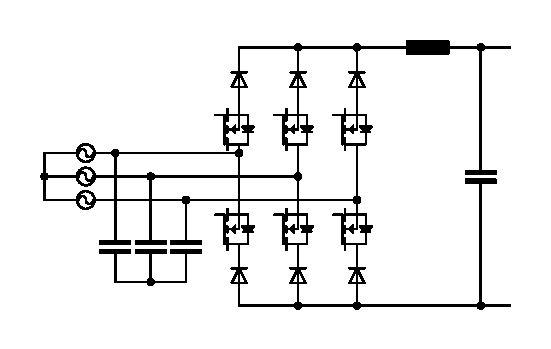
\includegraphics[width=0.7\linewidth]{content/Grafiken/SixSwitchBuck}
			\caption{Six Switch Buck PFC Rectifier}
			\label{fig:sixswitchbuck}
		\end{figure}
	
	\subsection{Swiss Rectifier}
		Bei dieser Topologie handelt es sich um die Integration des Tiefsetzstellers in die Schaltung des \gls{IAF}. Dazu wird die Induktivität im \gls{IVS} Pfad mit der des Tiefsetzstellers kombiniert und der Schalter des Tiefsetzstellers kann durch eine Diode ersetzt werden. Die Schaltung kann in Abbildung \ref{fig:swiss} gefunden werden und der \gls{IAF} wurde in Abbildung \ref{fig:iaf} bereits dargestellt. Durch die Einsparung des Schalters kann die Effizienz gesteigert werden. 
		\begin{figure}
			\centering
			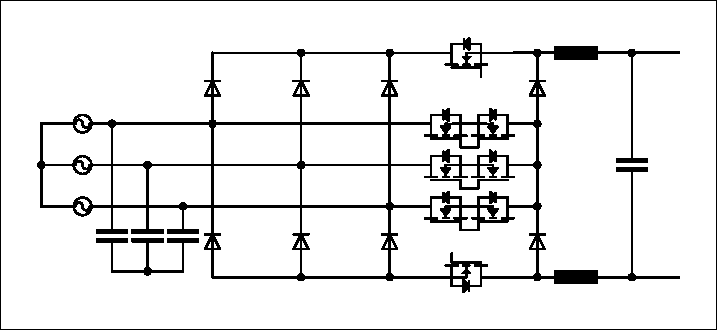
\includegraphics[width=0.7\linewidth]{content/Grafiken/Swiss}
			\caption{Swiss Rectifier}
			\label{fig:swiss}
		\end{figure}
		
	\subsection{2/3 PWM Buck \& Boost Current Source Rectifier}	
		Um einen breiteren Ausgangsspannungsbereich erzielen zu können wird der 6-Switch Buck durch einen Hochsetzsteller am Ausgang ergänzt. Dies ist in Abbildung \ref{fig:23pwmbuckboost} dargestellt. 
		\begin{figure}
			\centering
			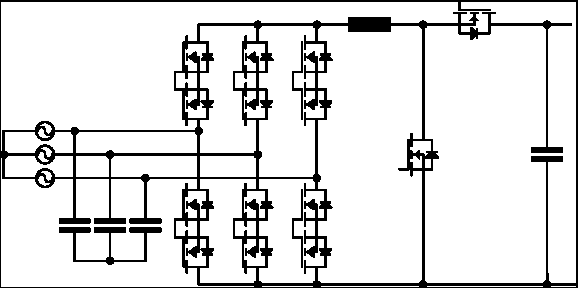
\includegraphics[width=0.7\linewidth]{content/Grafiken/23PWMBuckBoost}
			\caption{2/3 PWM Buck \& Boost Current Source Rectifier}
			\label{fig:23pwmbuckboost}
		\end{figure}
	\subsection{Trident Rectifier}
		Diese Topologie stammt vom 6-Switch Boost Rectifier ab, wobei an jeder Phasenhalbbrücke ein eigener Tiefsetzsteller angeschlossen wird. Somit besitzt jede Phase einen unabhängigen identischen Parallelen Aufbau zwischen AC und DC Pfad, siehe Abbildung \ref{fig:trident}. 
		\begin{figure}
			\centering
			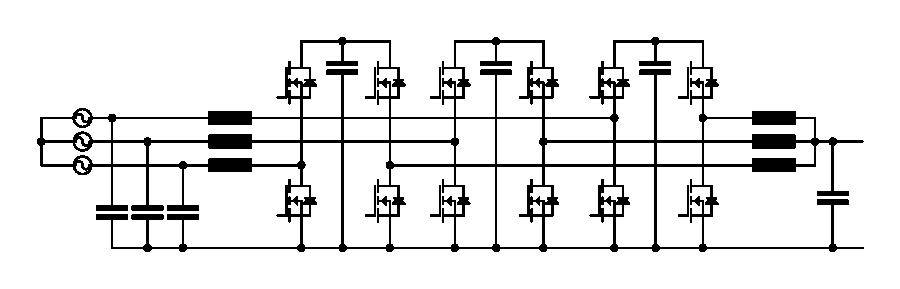
\includegraphics[width=0.7\linewidth]{content/Grafiken/Trident}
			\caption{Trident Rectifier}
			\label{fig:trident}
		\end{figure}
		
	\subsection{Y-Rectifier}
		Anstelle der Hoch- und Tiefstellenden Topologie wird hier umgekehrt Tief- und Hochgesetzt, dazu werden zwölf Halbleiterschalter genutzt. Es wird nur eine dreiphasige Drossel benötigt, welche zwischen den beiden Stellgliedern sitzt. Die Schaltung ist in Abbildung \ref{fig:y-rectifier} dargestellt.
		
	
		\begin{figure}
			\centering
			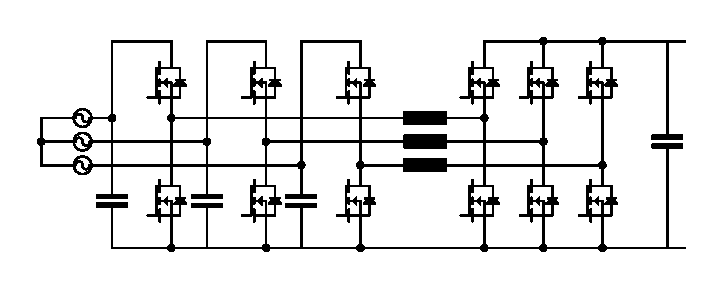
\includegraphics[width=0.7\linewidth]{content/Grafiken/Y-Rectifier}
			\caption{Y Rectifier}
			\label{fig:y-rectifier}
		\end{figure}

\section{Auswahl der Topologien}
Zur Eingrenzung des Lösungsraums wird zunächst eine Auflistung der möglichen Schaltungstopologien zum Anschluss an das dreiphasige Stromnetz erstellt, vgl. Tabelle \ref{tab:vorauswahl}. Die 15 aufgelisteten Topologien, begonnen mit dem in Abb. \ref{fig:B6DiodRect} dargestellten Diodengleichrichter, werden anhand der benötigten Induktivitäten, Dioden, Schalter und Stufen, sowie der Funktionsweise Hoch- bzw. Tiefstellend bewertet.\\
Tabelle \ref{tab:vorauswahl} zeigt, dass sich für eine engere Betrachtung die vier in grün hervorgehobenen Topologien eignen, da diese die im Vergleich wenigstens Induktivitäten und Halbleiter benötigen. Dioden sind aufgrund ihres simpleren Aufbaus günstiger als Leistungsschalter und fallen daher nicht so stark ins Gewicht. Die beiden anderen Topologien, 6-Switch Buck und Swiss Rectifier, werden in einer anderen Arbeit betrachtet.\\
Aufgrund der Komplexität der Schaltungen und benötigten Regelungen werden in dieser Arbeit der \gls{IAF} und \gls{B6PFC} betrachtet und die Ergebnisse für eine finale Bewertung aufbereitet.

\begin{table}
	\caption{Topologievergleich zur Vorauswahl}
	\label{tab:vorauswahl}
\begin{tabular}{|>{\centering\arraybackslash}p{3cm}|c|c|c|c|c|}
	\hline
	& Induktivitäten & Dioden & Schalter & Buck/Boost & Stufen \\
	\hline
	3-ΦDiode Bridge Rectifier & \cellcolor{yellow!25}3 &\cellcolor{red!25}6 &\cellcolor{green!25} 0 & \cellcolor{red!25}- & \cellcolor{green!25}1 \\
	\hline
	6-Switch Boost PFC Rectifier & \cellcolor{yellow!25}3 &\cellcolor{green!25} 0 & \cellcolor{green!25}6 & \cellcolor{red!25}Boost & \cellcolor{green!25}1 \\
	\hline
	Vienna Rectifier & \cellcolor{yellow!25}3 &\cellcolor{red!25}6 & \cellcolor{green!25}6 & \cellcolor{red!25}Boost & \cellcolor{green!25}1 \\
	\hline
	\cellcolor{green!10}6-Switch Buck PFC Rectifier & \cellcolor{green!25}1 &\cellcolor{red!25}6 &\cellcolor{green!25} 6 & \cellcolor{green!25}Buck & \cellcolor{green!25}1 \\
	\hline
	\cellcolor{green!10} \gls{IAF} & \cellcolor{green!25} 2 &\cellcolor{red!25}6 & \cellcolor{yellow!25}10 & \cellcolor{green!25}Buck & \cellcolor{red!25}2 \\
	\hline
	\cellcolor{green!10}Swiss Rectifier & \cellcolor{green!25}1 &\cellcolor{red!25}8 &\cellcolor{green!25} 8 & \cellcolor{green!25} Buck & \cellcolor{red!25}2 \\
	\hline
	\cellcolor{green!10} \gls{B6PFC} &\cellcolor{yellow!25}4 & \cellcolor{green!25} 0 &\cellcolor{green!25} 8 &\cellcolor{green!25} Boost/Buck & \cellcolor{red!25}2 \\
	\hline
	2/3 PWM Buck \& Boost Current Source Rectifier & \cellcolor{green!25} 1 & \cellcolor{green!25}0 & \cellcolor{yellow!25}14 & \cellcolor{green!25}Buck/Boost & \cellcolor{red!25}2 \\
	\hline
	Trident Rectifier & \cellcolor{red!25}6 &\cellcolor{green!25}0 & \cellcolor{yellow!25}12 & \cellcolor{green!25}Buck/Boost & \cellcolor{red!25}2 \\
	\hline
	Y-Rectifier & \cellcolor{yellow!25}3 &\cellcolor{green!25}0 & \cellcolor{yellow!25}12 &\cellcolor{green!25} Buck/Boost & \cellcolor{red!25}2 \\
	\hline
	3-Level Neutral Point Clamped & \cellcolor{yellow!25}3 &\cellcolor{red!25}6 & \cellcolor{yellow!25}12 & \cellcolor{red!25}Boost & \cellcolor{green!25}1 \\
	\hline
	3-Level Active Neutral Point Clamped  & \cellcolor{yellow!25}3 & \cellcolor{green!25}0 & \cellcolor{red!25}18 & \cellcolor{red!25}Boost & \cellcolor{green!25}1 \\
	\hline
	3-Level Active Neutral Point Clamped + Tiefsetzsteller & \cellcolor{yellow!25}4 &\cellcolor{green!25} 0 & \cellcolor{red!25}20 & \cellcolor{green!25}Boost/Buck & \cellcolor{red!25}2 \\
	\hline
	Three-Level Flying Capacitor (FC) Boost-Type Rectifier System & \cellcolor{yellow!25}3 & \cellcolor{green!25}0 & \cellcolor{yellow!25}12 & \cellcolor{red!25}Boost & \cellcolor{green!25}1 \\
	\hline
	Three-Level Flying Capacitor (FC + Tiefsetzsteller & \cellcolor{yellow!25}4 &\cellcolor{green!25}0 & \cellcolor{yellow!25}14 &\cellcolor{green!25} Boost/Buck &\cellcolor{red!25} 2 \\
	\hline
\end{tabular}
\end{table}
